%%% BEGIN fig:front-endpoint
\begin{figure}[htbp]
\centering
\begin{tikzpicture}[fd,
  fe heavy/.style={quark=#1,line width=1.25pt},
  fe heavy/.default=0.5,
  fe cA/.style={draw=blue!60!black},
  fe cB/.style={draw=orange!80!black},
  fe cS/.style={draw=green!45!black},
  fe lab/.style={font=\footnotesize}]
  % ======================= (a) the b-quark loop =======================
  \begin{scope}
    \coordinate (Hv) at (0,0); \coordinate (V1) at (2.0,1.15); \coordinate (V2) at (2.0,-1.15);
    \draw[scalar] (-1.55,0) -- (Hv);
    \draw[fe heavy,fe cA] (Hv) -- (V1);
    \draw[fe heavy,fe cS] (V1) -- (V2);
    \draw[fe heavy,fe cB] (V2) -- (Hv);
    \draw[photon] (V1) -- ++(30:1.85);
    \draw[photon] (V2) -- ++(-30:1.85);
    \foreach \p in {Hv,V1,V2} \node[vertex] at (\p) {};
    \node[anchor=east,inner sep=2pt] at (-1.55,0) {$h$};
    \node[anchor=south west,inner sep=1pt] at ($(V1)+(30:1.85)$) {$\gamma$};
    \node[anchor=north west,inner sep=1pt] at ($(V2)+(-30:1.85)$) {$\gamma$};
    \path[mom={$k_1$},mom pos=0.5] (V1) -- ++(30:1.85);
    \path[mom'={$k_2$},mom pos=0.5] (V2) -- ++(-30:1.85);
    \node[fe lab,text=blue!55!black,anchor=south east,inner sep=1.5pt] at ($(Hv)!0.5!(V1)$) {$n_1$ 共线};
    \node[fe lab,text=orange!65!black,anchor=north east,inner sep=1.5pt] at ($(Hv)!0.5!(V2)$) {$n_2$ 共线};
    \node[fe lab,text=green!35!black,anchor=west,inner sep=3pt] at ($(V1)!0.5!(V2)$) {软夸克};
    \node at (1.15,-3.25) {(a)\ $b$ 夸克圈：软夸克交换};
  \end{scope}
  % ======================= (b) third term H3 J (x) J (x) S =======================
  \begin{scope}[xshift=7.3cm]
    \coordinate (H) at (0,0);
    \coordinate (J1) at (1.75,1.05); \coordinate (J2) at (1.75,-1.05); \coordinate (S) at (3.15,0);
    \draw[scalar] (-1.55,0) -- (H);
    \draw[quark,fe cA] (H) -- (J1);
    \draw[quark,fe cB] (J2) -- (H);
    \draw[quark,fe cS] ($(J1)+(-58:0.3)$) -- (S);
    \draw[quark,fe cS] (S) -- ($(J2)+(58:0.3)$);
    \draw[photon] (J1) ++(30:0.62) -- ++(30:1.2);
    \draw[photon] (J2) ++(-30:0.62) -- ++(-30:1.2);
    \draw[hard blob] (H) circle[radius=0.42];
    \draw[jet blob,rotate around={30:(J1)}] (J1) ellipse[x radius=0.66cm,y radius=0.3cm];
    \draw[jetB blob,rotate around={-30:(J2)}] (J2) ellipse[x radius=0.66cm,y radius=0.3cm];
    \draw[soft blob] (S) circle[radius=0.36];
    \node at (H) {$H_3$};
    \node[font=\footnotesize] at (J1) {$J$};
    \node[font=\footnotesize] at (J2) {$J$};
    \node[font=\footnotesize] at (S) {$S$};
    \node[anchor=east,inner sep=2pt] at (-1.55,0) {$h$};
    \node[anchor=south west,inner sep=1pt] at ($(J1)+(30:1.82)$) {$\gamma(k_1)$};
    \node[anchor=north west,inner sep=1pt] at ($(J2)+(-30:1.82)$) {$\gamma(k_2)$};
    \node[fe lab,text=green!35!black,anchor=south west,inner sep=1pt] at ($(J1)!0.55!(S)+(0.08,0.02)$) {$\ell_+$};
    \node[fe lab,text=green!35!black,anchor=north west,inner sep=1pt] at ($(S)!0.45!(J2)+(0.08,-0.02)$) {$\ell_-$};
    \node[fe lab,text=red!60!black,anchor=west,align=left] at (3.65,0.1) {$\ell_\pm\to0$：\\端点发散};
    \node[fe lab,anchor=north west,align=left] at (3.62,-0.55) {重因子化条件\\$\Rightarrow$ 各项分别有限};
    \node[anchor=north] at (1.6,-2.33)
      {$H_3\int_{\color{red!65!black}0}\frac{\dd\ell_+}{\ell_+}\int_{\color{red!65!black}0}\frac{\dd\ell_-}{\ell_-}\,J(-M_h\ell_+)\,J(M_h\ell_-)\,S(\ell_+\ell_-)$};
    \node at (1.6,-3.25) {(b)\ 第三项 $H_3\,J\otimes J\otimes S$};
  \end{scope}
\end{tikzpicture}
\caption{$h\to\gamma\gamma$ 的 $b$ 夸克圈贡献的重整化端点因子化定理\cite{Liu:2019oav,Liu:2020wbn}（$\lambda=m_b/M_h$，一次质量插入，次领头幂次振幅）。
(a)~软夸克（绿）在两个光子共线扇区之间交换，与 Higgs 顶点相连的两条线分别与 $n_1$、$n_2$ 共线（蓝、橙）；箭头为费米子数流向，另一取向的圈图未画出；
(b)~因子化公式的第三项 $H_3\,J\otimes J\otimes S$：两个辐射喷注函数 $J$ 分别只依赖软夸克动量的分量 $\ell_+$、$\ell_-$，对 $\ell_\pm$ 的卷积在端点 $\ell_\pm\to0$ 发散；重因子化条件把端点发散在各项之间重新分配，给出各项分别有限的重整化定理，并再现领头双对数 $\mathcal M_0\frac{\hat L^2}2\,{}_2F_2(1,1;\frac32,2;-\frac{C_F\alpha_s}{8\pi}\hat L^2)$（全阶论证，VF-FRO-9）。}
\label{fig:front-endpoint}
\end{figure}
%%% END fig:front-endpoint

%%% BEGIN fig:front-gordan
\begin{figure}[htbp]
\centering
% Data: (a) D1=(2,0), D2=(1,2) (ex:front-gordan-2d), D3=(2.6,1.6) on the far side of the
% line D1D2; min-norm point of conv{D_j}: w=(8/5,4/5), |w|^2=16/5=D1.w=D2.w, D3.w=5.44;
% good cone {v: D_j.v>0} = directions between -26.57 deg (perp. to D2) and 90 deg (perp. to D1).
% (b) D3=(-1,-1): 1*D1+2*D2+4*D3=0 (closed polygon drawn at scale 0.4).
\begin{tikzpicture}[fd,
  fe vec/.style={draw,line width=0.9pt,-{Stealth[length=6pt,width=4.6pt]}},
  fe hull/.style={draw=gray!65,fill=gray!22,line width=0.6pt,line join=round},
  fe cone/.style={fill=green!9,draw=none},
  fe ray/.style={draw=green!45!black,line width=0.6pt,dash pattern=on 3pt off 2pt},
  fe wpt/.style={circle,fill=red!65!black,draw=none,inner sep=0pt,minimum size=4.6pt},
  fe lam/.style={draw=blue!60!black,line width=0.9pt,-{Stealth[length=6pt,width=4.6pt]}},
  fe lab/.style={font=\footnotesize}]
  % ======================= (a) good direction =======================
  \begin{scope}
    \fill[fe cone] (0,0) -- (-26.565:2.95) arc[start angle=-26.565,end angle=90,radius=2.95] -- cycle;
    \draw[fe ray] (0,0) -- (90:2.95);
    \draw[fe ray] (0,0) -- (-26.565:2.95);
    \draw[lcaxis,gray!55] (-1.15,0) -- (3.35,0);
    \draw[lcaxis,gray!55] (0,-1.75) -- (0,3.3);
    % supporting line v.w = |w|^2 through D1, D2
    \draw[gray!60!black,densely dotted,line width=0.6pt] ($(2,0)!-0.45!(1,2)$) -- ($(2,0)!1.32!(1,2)$);
    \draw[fe hull] (2,0) -- (1,2) -- (2.6,1.6) -- cycle;
    \draw[fe vec] (0,0) -- (2,0);
    \draw[fe vec] (0,0) -- (1,2);
    \draw[fe vec] (0,0) -- (2.6,1.6);
    \draw[red!65!black,line width=0.7pt,dash pattern=on 2.5pt off 1.8pt] (0,0) -- (1.6,0.8);
    % right-angle mark at w on the D1 side (face direction (1,-2)/sqrt5, normal (2,1)/sqrt5),
    % away from the arrow D3 which passes just above w
    \draw[red!65!black,line width=0.5pt] ($(1.6,0.8)+(0.0894,-0.1789)$) -- ++(-0.1789,-0.0894) -- ++(-0.0894,0.1789);
    \node[fe wpt] at (1.6,0.8) {};
    \node[anchor=north east,inner sep=1.5pt] at (2.02,-0.03) {$D_1$};
    \node[anchor=east,inner sep=2pt] at (0.98,2.05) {$D_2$};
    \node[anchor=west,inner sep=2pt] at (2.62,1.62) {$D_3$};
    \node[inner sep=1pt,text=red!60!black] at (1.27,0.42) {$w$};
    \node[fill=white,fill opacity=0.85,text opacity=1,inner sep=1pt] at (0,0) {};
    \node[anchor=north east,inner sep=1.5pt] at (0,0) {$0$};
    \node[fe lab,text=green!35!black,anchor=south,align=center] at (1.5,2.82) {好方向锥 $\{v:D_j\cdot v>0\}$};
    \node[fe lab,text=gray!40!black,anchor=north west] at (2.38,-0.62) {$v\cdot w=|w|^2$};
    \node at (1.05,-2.25) {(a)\ $D_j\cdot w\ge|w|^2$：好方向};
  \end{scope}
  % ======================= (b) Landau point =======================
  \begin{scope}[xshift=7.1cm]
    \draw[lcaxis,gray!55] (-1.75,0) -- (2.75,0);
    \draw[lcaxis,gray!55] (0,-1.75) -- (0,3.3);
    \draw[fe hull] (2,0) -- (1,2) -- (-1,-1) -- cycle;
    \draw[fe vec] (0,0) -- (2,0);
    \draw[fe vec] (0,0) -- (1,2);
    \draw[fe vec] (0,0) -- (-1,-1);
    \node[circle,fill=black,draw=none,inner sep=0pt,minimum size=3.6pt] at (0,0) {};
    \node[anchor=north west,inner sep=1.5pt] at (1.98,-0.03) {$D_1$};
    \node[anchor=east,inner sep=2pt] at (0.98,2.05) {$D_2$};
    \node[anchor=north east,inner sep=1.5pt] at (-1,-1) {$D_3$};
    \node[anchor=south east,inner sep=1.5pt] at (-0.05,0.05) {$0$};
    % closed polygon of the weighted vectors (scale 0.4)
    \begin{scope}[shift={(2.85,0.55)},scale=0.4]
      \draw[fe lam] (0,0) -- (2,0);
      \draw[fe lam] (2,0) -- (4,4);
      \draw[fe lam] (4,4) -- (0,0);
      \node[fe lab,anchor=north,inner sep=2pt] at (1,0) {$\lambda_1D_1$};
      \node[fe lab,anchor=west,inner sep=2pt] at (3,2) {$\lambda_2D_2$};
      \node[fe lab,anchor=south east,inner sep=1pt] at (2,2.05) {$\lambda_3D_3$};
    \end{scope}
    \node[fe lab,align=center,anchor=north] at (3.6,-0.35) {$\lambda=(1,2,4)$\\[1pt]$\sum_j\lambda_jD_j=0$};
    \node at (1.25,-2.25) {(b)\ Landau 点：无好方向};
  \end{scope}
\end{tikzpicture}
\caption{Gordan 二择一定理（1873）\cite{Gordan1873}：对有限个对偶矢量 $D_j$，要么存在好方向 $v$（$D_j\cdot v>0$，可取凸包中范数最小的点 $w$，并有 $D_j\cdot w\ge|w|^2$），要么存在 Landau 点（$\lambda_j\ge0$ 不全为零、$\sum_j\lambda_jD_j=0$），二者恰有其一。
(a)~$D_1=(2,0)$、$D_2=(1,2)$ 与 $D_3$ 的凸包（灰）不含原点，最小范数点 $w=(\frac85,\frac45)$ 落在面 $D_1D_2$ 上（$D_1\cdot w=D_2\cdot w=|w|^2$），位于好方向锥（绿）之内；
(b)~换成 $D_3=(-1,-1)$ 后凸包含原点，$1\cdot D_1+2\cdot D_2+4\cdot D_3=0$（蓝色闭合折线），不存在好方向。
在 Collins\cite{Collins:2020euz}（2020，预印本）的符号条件下，积分围道在 $w_S$ 被钳住当且仅当存在 Landau 点（VF-FRO-1，VF-FRO-2）。}
\label{fig:front-gordan}
\end{figure}
%%% END fig:front-gordan

%%% BEGIN fig:front-regions-polytope
\begin{figure}[htbp]
\centering
% Schematic only (no data): a Newton polygon with lower chain S, C1, H, C2 (the adjacency
% S-C1-H-C2 is that of the four essential facets of the one-loop off-shell triangle;
% the 2D shape itself is not a projection of that polytope).
\begin{tikzpicture}[fd,x=0.56cm,y=0.56cm,
  fe poly/.style={draw=gray!60,fill=gray!10,line width=0.6pt,line join=round},
  fe pt/.style={circle,fill=black,draw=none,inner sep=0pt,minimum size=3.4pt},
  fe ipt/.style={circle,fill=gray!55,draw=none,inner sep=0pt,minimum size=3pt},
  fe facet/.style={line width=1.7pt,line cap=round},
  fe normal/.style={draw,line width=0.6pt,-{Stealth[length=4pt,width=3.4pt]}},
  fe sign/.style={circle,fill=white,line width=0.7pt,inner sep=0pt,minimum size=8.5pt,font=\scriptsize\bfseries},
  fe lab/.style={font=\footnotesize}]
  % ======================= (a) Euclidean type =======================
  \begin{scope}
    \draw[lcaxis] (-0.7,-0.7) -- (9.4,-0.7) node[below left=1pt,fe lab] {$x$ 的指数（投影）};
    \draw[lcaxis] (-0.7,-0.7) -- (-0.7,6.1) node[right=1pt,fe lab] {$t$ 的指数};
    \draw[fe poly] (0,3) -- (1,1) -- (3,0) -- (6,0) -- (8,1) -- (8,3) -- (6,5) -- (2,5) -- cycle;
    \draw[fe facet,green!45!black] (0,3) -- (1,1);
    \draw[fe facet,blue!60!black] (1,1) -- (3,0);
    \draw[fe facet,black!65] (3,0) -- (6,0);
    \draw[fe facet,orange!80!black] (6,0) -- (8,1);
    \foreach \p in {(0,3),(1,1),(3,0),(6,0),(8,1),(8,3),(6,5),(2,5),(4,0)} \node[fe pt] at \p {};
    \foreach \p in {(2,2),(3,3),(5,2),(6,3),(4,4),(2,4)} \node[fe ipt] at \p {};
    % inward normals of the lower facets (r_{n+1}>0)
    \draw[fe normal,green!45!black] (0.5,2) -- ++(0.894*1.3,0.447*1.3);
    \draw[fe normal,blue!60!black] (2,0.5) -- ++(0.447*1.3,0.894*1.3);
    \draw[fe normal,black!65] (4.5,0) -- ++(0,1.3) node[above,fe lab,inner sep=1pt] {$r$};
    \draw[fe normal,orange!80!black] (7,0.5) -- ++(-0.447*1.3,0.894*1.3);
    \node[fe lab,text=green!40!black,anchor=east] at (0.38,1.75) {$S$};
    \node[fe lab,text=blue!55!black,anchor=north east,inner sep=1pt] at (1.9,0.42) {$C_1$};
    \node[fe lab,anchor=north,inner sep=1.5pt] at (4.5,-0.02) {$H$};
    \node[fe lab,text=orange!65!black,anchor=north west,inner sep=1pt] at (7.1,0.42) {$C_2$};
    \node at (4.35,-2.75) {(a)\ 欧氏型：系数全正};
  \end{scope}
  % ======================= (b) Minkowski kinematics =======================
  \begin{scope}[xshift=6.0cm]
    \draw[lcaxis] (-0.7,-1.6) -- (9.4,-1.6);
    \draw[lcaxis] (-0.7,-1.6) -- (-0.7,6.1);
    \draw[fe poly] (0,3) -- (1,1) -- (3,0) -- (6,0) -- (8,1) -- (8,3) -- (6,5) -- (2,5) -- cycle;
    \draw[fe facet,green!45!black,line width=1.1pt] (0,3) -- (1,1);
    \draw[fe facet,blue!60!black,line width=1.1pt] (1,1) -- (3,0);
    \draw[fe facet,black!65,line width=1.1pt] (3,0) -- (6,0);
    \draw[fe facet,orange!80!black,line width=1.1pt] (6,0) -- (8,1);
    \foreach \p in {(0,3),(1,1),(8,1),(8,3),(6,5),(2,5)} \node[fe pt] at \p {};
    \foreach \p in {(2,2),(3,3),(5,2),(6,3),(4,4),(2,4)} \node[fe ipt] at \p {};
    % new lower facet after dissection (drawn first, the sign circles cover its ends)
    \draw[red!65!black,line width=1.1pt,dash pattern=on 3.5pt off 2pt] (3,0) -- (4.5,-1) -- (6,0);
    \node[circle,draw=red!65!black,fill=red!15,line width=0.7pt,inner sep=0pt,minimum size=4.4pt] at (4.5,-1) {};
    % opposite-sign monomials on the facet H
    \node[fe sign,draw=blue!60!black] at (3,0) {$+$};
    \node[fe sign,draw=red!65!black] at (6,0) {$-$};
    \draw[red!65!black,line width=0.6pt,{Stealth[length=3.6pt]}-{Stealth[length=3.6pt]}] (3.5,0.6) -- node[above,fe lab,inner sep=1.5pt] {相消} (5.5,0.6);
    \node[fe lab,text=red!60!black,anchor=west] at (5.3,-1.05) {剖分后的新面：隐藏区域（如 Glauber）};
    % inset: parameter space with an interior pinch
    \begin{scope}[shift={(10.3,2.1)}]
      \fill[gray!8] (0,0) rectangle (3.5,3.5);
      \draw[lcaxis] (0,0) -- (3.95,0) node[below,fe lab] {$x_i$};
      \draw[lcaxis] (0,0) -- (0,3.95) node[left,fe lab] {$x_j$};
      \draw[red!65!black,line width=0.8pt] plot[domain=0.55:3.5,samples=40,smooth] (\x,{1.9/\x});
      \draw[red!65!black,line width=1pt] (1.6,1.1875) ++(-0.24,-0.24) -- ++(0.48,0.48) ++(0,-0.48) -- ++(-0.48,0.48);
      \node[fe lab,text=red!60!black,anchor=south west,inner sep=1pt] at (1.85,1.3) {钳夹};
      \node[fe lab,align=center,anchor=north] at (1.75,-0.5) {参数空间：内部钳夹，\\而非端点奇异};
    \end{scope}
    \node at (6.6,-2.75) {(b)\ Minkowski 运动学：异号项（如三圈非平面 $2\to2$）};
  \end{scope}
\end{tikzpicture}
\caption{区域方法的几何（示意）：(a)~当 $\mathcal U+\mathcal F$ 的系数全为正（欧氏型）时，区域对应 Newton 多面体的本质下表面（$S$、$C_1$、$H$、$C_2$，颜色同约化图中的软、共线与硬子图），法向量 $r$（$r_{n+1}>0$）给出各 Feynman 参数的标度 $x_i\to t^{r_i}x_i$；
(b)~Minkowski 运动学中异号项的相消在参数空间内部产生钳夹，标准的下表面算法漏掉相应区域，沿奇异轨迹剖分后出现新的面（红色虚线）——“隐藏区域”\cite{Gardi:2024axt}。
“区域 $=$ 下表面”作为一般陈述在 Minkowski 运动学中不成立。}
\label{fig:front-regions-polytope}
\end{figure}
%%% END fig:front-regions-polytope

%%% BEGIN fig:front-yukawa-pdf
\begin{figure}[htbp]
\centering
% Curves: VF-FRO-10, f/a_lambda=(1-xi)[ln(mu^2/Delta)-1+(m_q+xi m_p)^2/Delta],
% Delta=xi m_s^2+(1-xi)m_q^2-xi(1-xi)m_p^2, m_q=0.3, m_p=1.0, m_s=1.5 GeV (starter code of
% FIGURES_INDEX_v2 N17; ymin/ymax widened so that no curve is clipped: f(0.001;2.5)=4.22).
% Zeros: mu=0.8: xi=0.26403; mu=1.2: xi=0.56737 (mpmath findroot); mu=2.5: min f=7.7e-4>0.
% Minimum of the mu=0.8 curve: -0.351 at xi=0.58 (labels of the zeros placed below it).
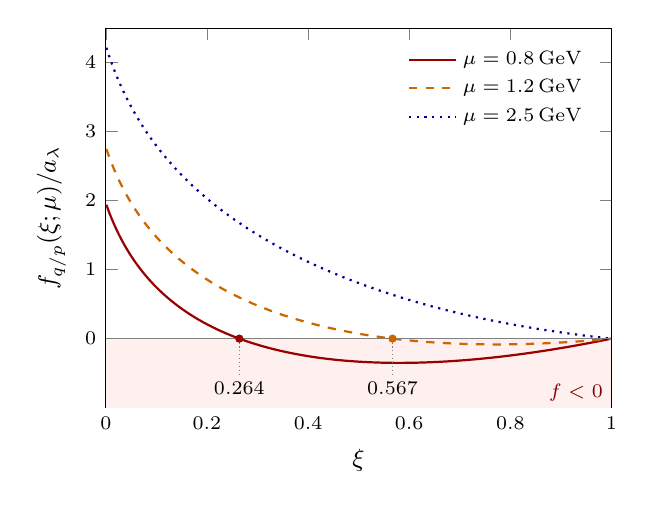
\begin{tikzpicture}
\begin{axis}[width=0.66\textwidth,height=6.4cm,xmin=0,xmax=1,ymin=-1.0,ymax=4.5,
  xlabel={$\xi$},ylabel={$f^{\MSbar}_{q/p}(\xi;\mu)/a_\lambda$},
  xtick={0,0.2,0.4,0.6,0.8,1},ytick={0,1,2,3,4},
  tick label style={font=\scriptsize},label style={font=\small},
  legend style={font=\scriptsize,draw=none,fill=none,at={(0.97,0.97)},anchor=north east},
  legend cell align=left]
\fill[red!6] (axis cs:0,-1.0) rectangle (axis cs:1,0);
\addplot[domain=0.001:0.999,samples=200,thick,red!60!black]{(1-x)*(ln(0.8^2/(2.25*x+0.09*(1-x)-x*(1-x)))-1+(0.3+x)^2/(2.25*x+0.09*(1-x)-x*(1-x)))};
\addlegendentry{$\mu=0.8\,\mathrm{GeV}$}
\addplot[domain=0.001:0.999,samples=200,thick,dashed,orange!80!black]{(1-x)*(ln(1.2^2/(2.25*x+0.09*(1-x)-x*(1-x)))-1+(0.3+x)^2/(2.25*x+0.09*(1-x)-x*(1-x)))};
\addlegendentry{$\mu=1.2\,\mathrm{GeV}$}
\addplot[domain=0.001:0.999,samples=200,thick,dotted,blue!60!black]{(1-x)*(ln(2.5^2/(2.25*x+0.09*(1-x)-x*(1-x)))-1+(0.3+x)^2/(2.25*x+0.09*(1-x)-x*(1-x)))};
\addlegendentry{$\mu=2.5\,\mathrm{GeV}$}
\draw[gray,thin] (axis cs:0,0) -- (axis cs:1,0);
\draw[gray,densely dotted] (axis cs:0.264,0) -- (axis cs:0.264,-0.56);
\draw[gray,densely dotted] (axis cs:0.567,0) -- (axis cs:0.567,-0.56);
\fill[red!60!black] (axis cs:0.264,0) circle[radius=1.5pt];
\fill[orange!80!black] (axis cs:0.567,0) circle[radius=1.5pt];
\node[font=\scriptsize,anchor=north,inner sep=1.5pt] at (axis cs:0.264,-0.56) {$0.264$};
\node[font=\scriptsize,anchor=north,inner sep=1.5pt] at (axis cs:0.567,-0.56) {$0.567$};
\node[font=\scriptsize,text=red!50!black,anchor=south east,inner sep=2pt] at (axis cs:0.995,-1.0) {$f<0$};
\end{axis}
\end{tikzpicture}
\caption{Yukawa 模型中单圈 $\MSbar$ “夸克在核子中”的分布（$m_q=0.3\,\mathrm{GeV}$、$m_p=1.0\,\mathrm{GeV}$、$m_s=1.5\,\mathrm{GeV}$，纵轴以 $a_\lambda=\lambda^2/(16\pi^2)$ 为单位）\cite{CollinsRogersSato2022}：$\mu=0.8\,\mathrm{GeV}$ 时 $\xi>0.264$ 处为负，$\mu=1.2\,\mathrm{GeV}$ 时 $\xi>0.567$ 处为负，$\mu=2.5\,\mathrm{GeV}$ 时处处为正（曲线由 VF-FRO-10 的单圈公式计算）。
“$\MSbar$ 分布在所有标度上非负”因而不成立；足够大标度上的正定性只有部分论证（\cref{prop:front-positivity-large-scale}），一般陈述仍是猜想（\cref{conj:pdf-positivity}）。}
\label{fig:front-yukawa-pdf}
\end{figure}
%%% END fig:front-yukawa-pdf
